\documentclass[12pt]{article}
\usepackage{tikz}
\usepackage{amsmath}
\usepackage{geometry}
\usepackage{graphicx}
\geometry{a4paper, margin=1in}

\tikzset{
	lattice node/.style={
		draw, 
		rounded corners, 
		fill=white, 
		align=center, 
		inner sep=4pt, 
		minimum width=1.4cm,
		font=\footnotesize
	},
	pos node/.style={lattice node, fill=blue!10},
	neg node/.style={lattice node, fill=red!10},
	edge style/.style={thick, gray!50}
}

\begin{document}
	
	\begin{center}
		\LARGE \textbf{Geometric and Lattice Visualizations of}\\
		\textbf{Euler's Pentagonal Number Theorem Expansions}\\
		\large $\prod_{k=1}^n (1-q^k)$
	\end{center}
	
	\vspace{0.5cm}
	
	% =========================================================================
	% PART 1: SPATIAL GEOMETRY
	% =========================================================================
	\section*{Part 1: Spatial Geometry ($n=1$ to $3$)}
	
	\subsection*{1D Geometry: $n=1 \implies 1-q$}
	A 1D line segment of length 1. We remove a segment of length $q$.
	\vspace{0.3cm}
	\begin{center}
		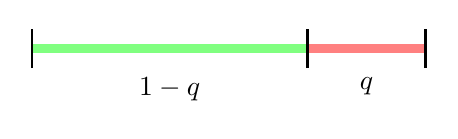
\begin{tikzpicture}[scale=5]
			\draw[thick] (0,0) -- (1,0);
			\draw[line width=3pt, green!50] (0,0) -- (0.7,0);
			\draw[line width=3pt, red!50] (0.7,0) -- (1,0);
			\draw[thick] (0,-0.05) -- (0,0.05);
			\draw[thick] (0.7,-0.05) -- (0.7,0.05);
			\draw[thick] (1,-0.05) -- (1,0.05);
			\node[below] at (0.35, -0.05) {$1-q$};
			\node[below] at (0.85, -0.05) {$q$};
		\end{tikzpicture}
	\end{center}
	
	\subsection*{2D Geometry: $n=2 \implies (1-q)(1-q^2) = 1 - q - q^2 + q^3$}
	A square where we remove a vertical strip $q$ and a horizontal strip $q^2$. The intersection $q^3$ is added back.
	\vspace{0.3cm}
	\begin{center}
		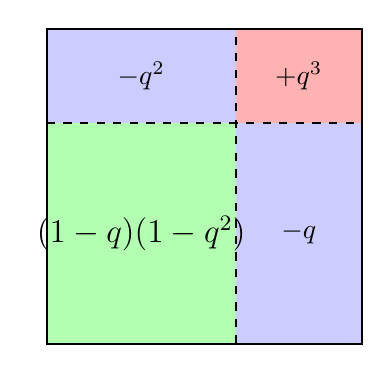
\begin{tikzpicture}[scale=4]
			\fill[green!30] (0,0) rectangle (0.6,0.7);
			\fill[blue!20] (0.6,0) rectangle (1,0.7);
			\fill[blue!20] (0,0.7) rectangle (0.6,1);
			\fill[red!30] (0.6,0.7) rectangle (1,1);
			\draw[thick] (0,0) rectangle (1,1);
			\draw[dashed, thick] (0.6,0) -- (0.6,1);
			\draw[dashed, thick] (0,0.7) -- (1,0.7);
			
			\node at (0.3, 0.35) {\large $(1-q)(1-q^2)$};
			\node at (0.8, 0.35) {$-q$};
			\node at (0.3, 0.85) {$-q^2$};
			\node at (0.8, 0.85) {\textbf{$+q^3$}};
		\end{tikzpicture}
	\end{center}
	
	\subsection*{3D Geometry: $n=3 \implies \prod_{k=1}^3 (1-q^k) = 1 - q - q^2 + q^4 + q^5 - q^6$}
	The intersection volume $q^3$ cancels identically with the third spatial slice $q^3$.
	\vspace{0.3cm}
	\begin{center}
		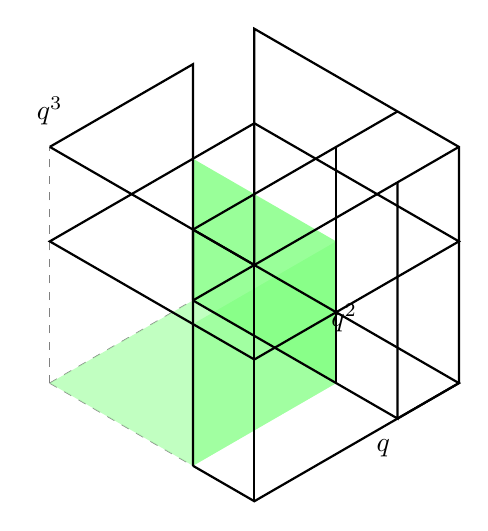
\begin{tikzpicture}[
			scale=3, 
			x={(0.866cm,-0.5cm)}, 
			y={(0.866cm,0.5cm)}, 
			z={(0cm,1cm)}
			]
			\draw[dashed, gray] (0,0,0) -- (1,0,0);
			\draw[dashed, gray] (0,0,0) -- (0,1,0);
			\draw[dashed, gray] (0,0,0) -- (0,0,1);
			
			\fill[green!30, opacity=0.8] (0,0,0) -- (0.7,0,0) -- (0.7,0.7,0) -- (0,0.7,0) -- cycle;
			\fill[green!40, opacity=0.8] (0.7,0,0) -- (0.7,0.7,0) -- (0.7,0.7,0.6) -- (0.7,0,0.6) -- cycle;
			\fill[green!50, opacity=0.8] (0,0.7,0) -- (0.7,0.7,0) -- (0.7,0.7,0.6) -- (0,0.7,0.6) -- cycle;
			
			\draw[thick] (0.7,0,0) -- (1,0,0) -- (1,1,0) -- (0,1,0) -- (0,0.7,0);
			\draw[thick] (1,0,0) -- (1,0,1);
			\draw[thick] (1,1,0) -- (1,1,1) -- (0,1,1) -- (0,1,0);
			\draw[thick] (0,0.7,0) -- (0,0.7,1) -- (0,0,1);
			\draw[thick] (1,0,1) -- (1,1,1);
			\draw[thick] (0,0,1) -- (1,0,1);
			
			\draw[thick] (0.7,0,0) -- (0.7,0,1) -- (0.7,1,1);
			\draw[thick] (0.7,0,1) -- (1,0,1);
			\draw[thick] (0,0.7,0) -- (1,0.7,0) -- (1,0.7,1);
			\draw[thick] (1,0.7,0) -- (1,1,0);
			\draw[thick] (0,0,0.6) -- (1,0,0.6) -- (1,1,0.6) -- (0,1,0.6) -- cycle;
			\draw[thick] (0.7,0.7,0) -- (0.7,0.7,1);
			
			\node[right] at (1.05, 0.5, 0) {$q$};
			\node[left]  at (0.5, 1.05, 0) {$q^2$};
			\node[above] at (0, 0, 1.05) {$q^3$};
		\end{tikzpicture}
	\end{center}
	
	\newpage
	% =========================================================================
	% PART 2: COMBINATORIAL LATTICES
	% =========================================================================
	\section*{Part 2: Combinatorial Lattices ($n=1$ to $5$)}
	Blue nodes represent geometric additions ($+$). Red nodes represent subtractions ($-$). 
	
	\vspace{0.5cm}
	
	\subsection*{1 \& 2. Lattices for $n=1$ and $n=2$}
	\begin{center}
		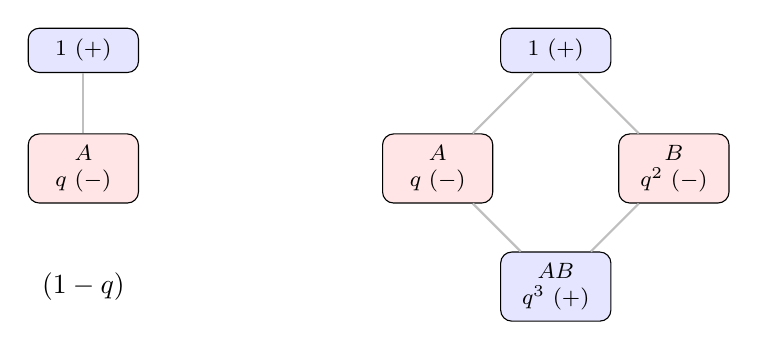
\begin{tikzpicture}
			% n=1
			\node[pos node] (0_1)  at (-4, 0) {$1$ ($+$)};
			\node[neg node] (A_1)  at (-4, -1.5) {$A$\\$q$ ($-$)\vphantom{$^2$}};
			\draw[edge style] (0_1) -- (A_1);
			\node at (-4, -3) {$(1-q)$};
			
			% n=2
			\node[pos node] (0)  at (2, 0) {$1$ ($+$)};
			\node[neg node] (A)  at (0.5, -1.5) {$A$\\$q$ ($-$)\vphantom{$^2$}};
			\node[neg node] (B)  at (3.5, -1.5) {$B$\\$q^2$ ($-$)\vphantom{$^2$}};
			\node[pos node] (AB) at (2, -3) {$AB$\\$q^3$ ($+$)};
			
			\draw[edge style] (0) -- (A); \draw[edge style] (0) -- (B);
			\draw[edge style] (A) -- (AB); \draw[edge style] (B) -- (AB);
		\end{tikzpicture}
	\end{center}
	
	\vspace{0.5cm}
	
	\subsection*{3. Lattice for $n=3$: $1 - q - q^2 + q^4 + q^5 - q^6$}
	\begin{center}
		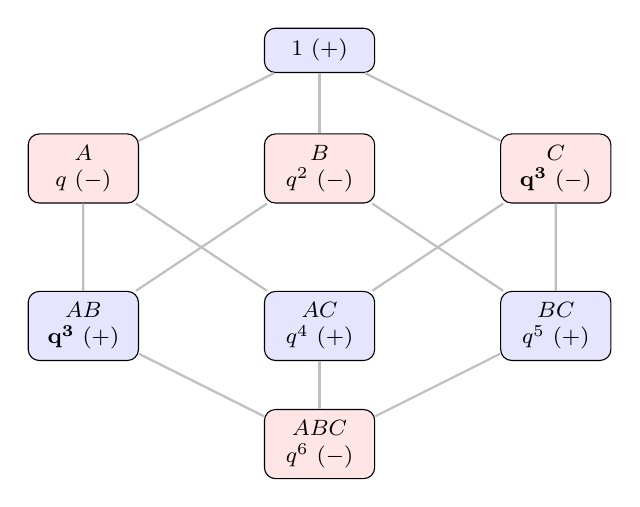
\begin{tikzpicture}[xscale=1.5]
			\node[pos node] (0)  at (0, 0) {$1$ ($+$)};
			\node[neg node] (A)  at (-2, -1.5) {$A$\\$q$ ($-$)\vphantom{$^2$}};
			\node[neg node] (B)  at (0, -1.5) {$B$\\$q^2$ ($-$)\vphantom{$^2$}};
			\node[neg node] (C)  at (2, -1.5) {$C$\\$\mathbf{q^3}$ ($-$)\vphantom{$^2$}};
			\node[pos node] (AB) at (-2, -3.5) {$AB$\\$\mathbf{q^3}$ ($+$)};
			\node[pos node] (AC) at (0, -3.5) {$AC$\\$q^4$ ($+$)};
			\node[pos node] (BC) at (2, -3.5) {$BC$\\$q^5$ ($+$)};
			\node[neg node] (ABC) at (0, -5) {$ABC$\\$q^6$ ($-$)\vphantom{$^2$}};
			
			\foreach \u/\v in {0/A,0/B,0/C,A/AB,A/AC,B/AB,B/BC,C/AC,C/BC,AB/ABC,AC/ABC,BC/ABC} \draw[edge style] (\u) -- (\v);
		\end{tikzpicture}
	\end{center}
	
	\newpage
	\subsection*{4. Lattice for $n=4$: $1 - q - q^2 + 2q^5 - q^8 - q^9 + q^{10}$}
	\begin{center}
		\resizebox{0.9\textwidth}{!}{
			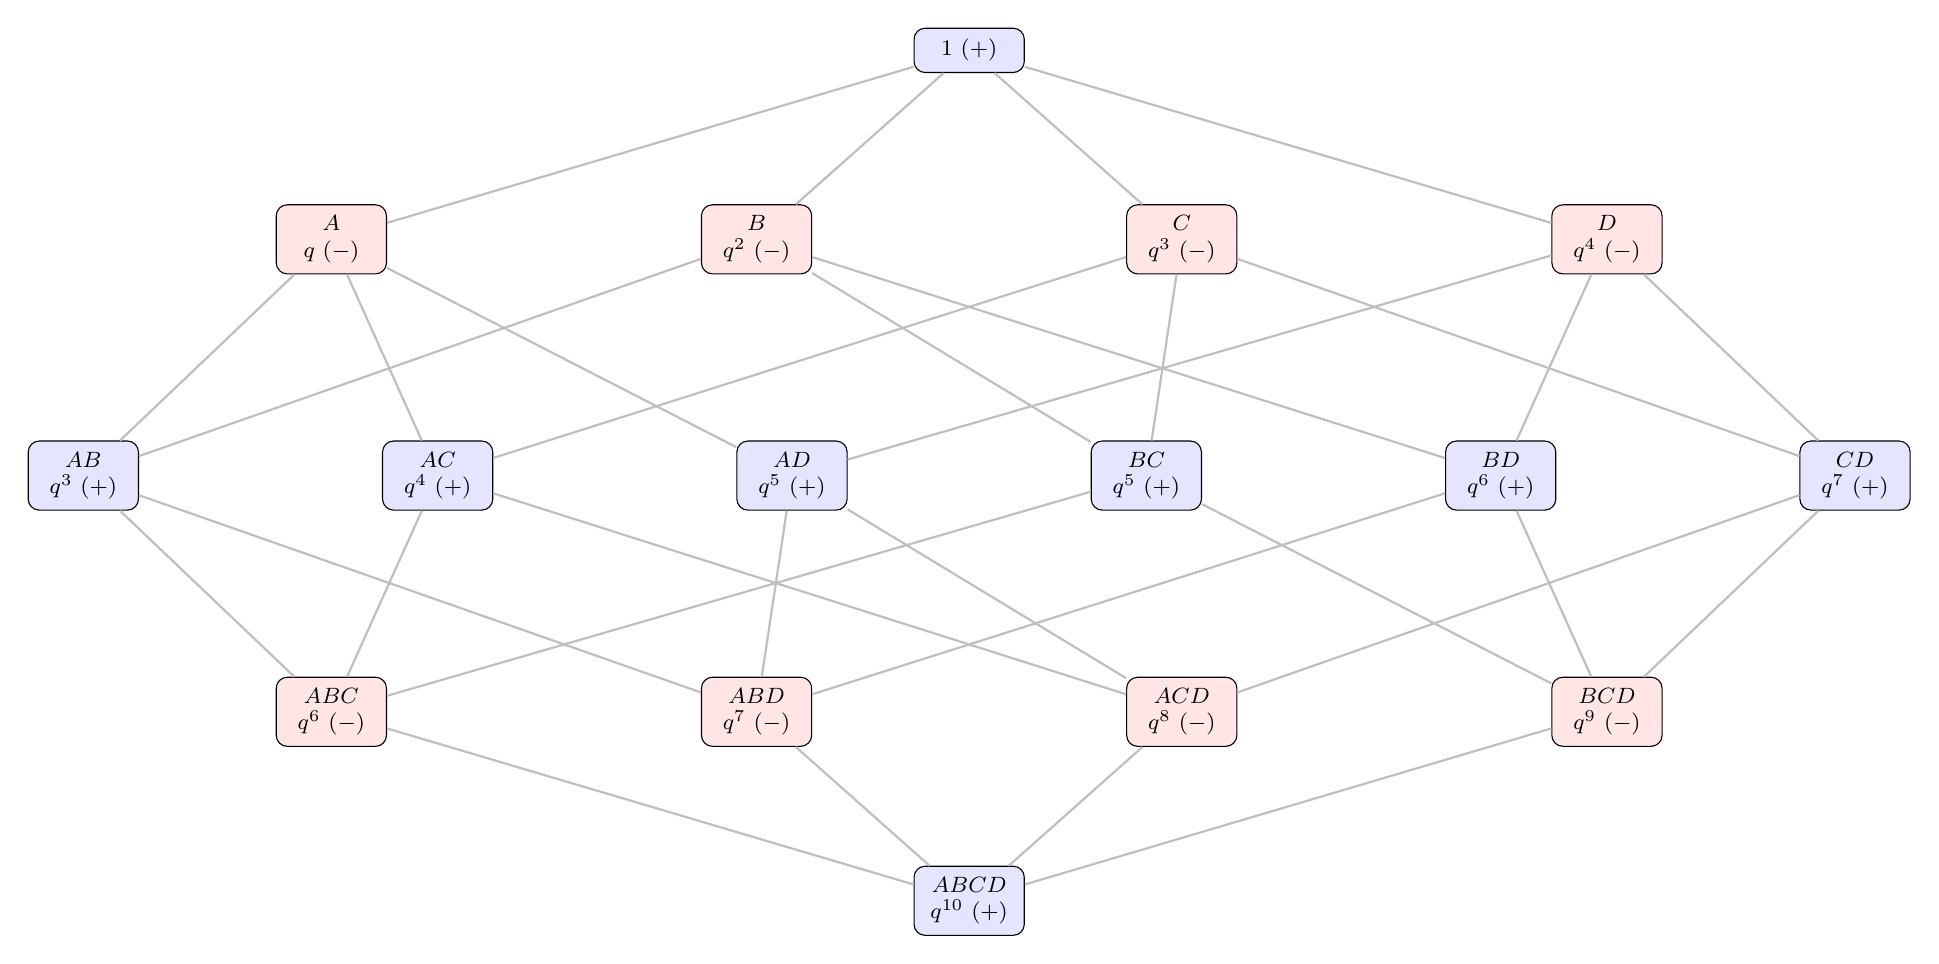
\begin{tikzpicture}[xscale=1.8, yscale=1.2]
				\node[pos node] (0) at (0, 0) {$1$ ($+$)};
				
				\node[neg node] (A) at (-4.5, -2) {$A$\\$q$ ($-$)\vphantom{$^2$}};
				\node[neg node] (B) at (-1.5, -2) {$B$\\$q^2$ ($-$)\vphantom{$^2$}};
				\node[neg node] (C) at (1.5, -2) {$C$\\$q^3$ ($-$)\vphantom{$^2$}};
				\node[neg node] (D) at (4.5, -2) {$D$\\$q^4$ ($-$)\vphantom{$^2$}};
				
				\node[pos node] (AB) at (-6.25, -4.5) {$AB$\\$q^3$ ($+$)};
				\node[pos node] (AC) at (-3.75, -4.5) {$AC$\\$q^4$ ($+$)};
				\node[pos node] (AD) at (-1.25, -4.5) {$AD$\\$q^5$ ($+$)};
				\node[pos node] (BC) at (1.25, -4.5) {$BC$\\$q^5$ ($+$)};
				\node[pos node] (BD) at (3.75, -4.5) {$BD$\\$q^6$ ($+$)};
				\node[pos node] (CD) at (6.25, -4.5) {$CD$\\$q^7$ ($+$)};
				
				\node[neg node] (ABC) at (-4.5, -7) {$ABC$\\$q^6$ ($-$)\vphantom{$^2$}};
				\node[neg node] (ABD) at (-1.5, -7) {$ABD$\\$q^7$ ($-$)\vphantom{$^2$}};
				\node[neg node] (ACD) at (1.5, -7) {$ACD$\\$q^8$ ($-$)\vphantom{$^2$}};
				\node[neg node] (BCD) at (4.5, -7) {$BCD$\\$q^9$ ($-$)\vphantom{$^2$}};
				
				\node[pos node] (ABCD) at (0, -9) {$ABCD$\\$q^{10}$ ($+$)};
				
				\foreach \u/\v in {0/A,0/B,0/C,0/D} \draw[edge style] (\u) -- (\v);
				\foreach \u/\v in {A/AB,A/AC,A/AD,B/AB,B/BC,B/BD,C/AC,C/BC,C/CD,D/AD,D/BD,D/CD} \draw[edge style] (\u) -- (\v);
				\foreach \u/\v in {AB/ABC,AB/ABD,AC/ABC,AC/ACD,AD/ABD,AD/ACD,BC/ABC,BC/BCD,BD/ABD,BD/BCD,CD/ACD,CD/BCD} \draw[edge style] (\u) -- (\v);
				\foreach \u/\v in {ABC/ABCD,ABD/ABCD,ACD/ABCD,BCD/ABCD} \draw[edge style] (\u) -- (\v);
			\end{tikzpicture}
		}
	\end{center}
	
	\newpage
	\subsection*{5. Lattice for $n=5$: $1 - q - q^2 + q^5 + q^6 + q^7 - q^8 - q^9 - q^{10} + q^{13} + q^{14} - q^{15}$}
	\begin{center}
		\resizebox{\textwidth}{!}{
			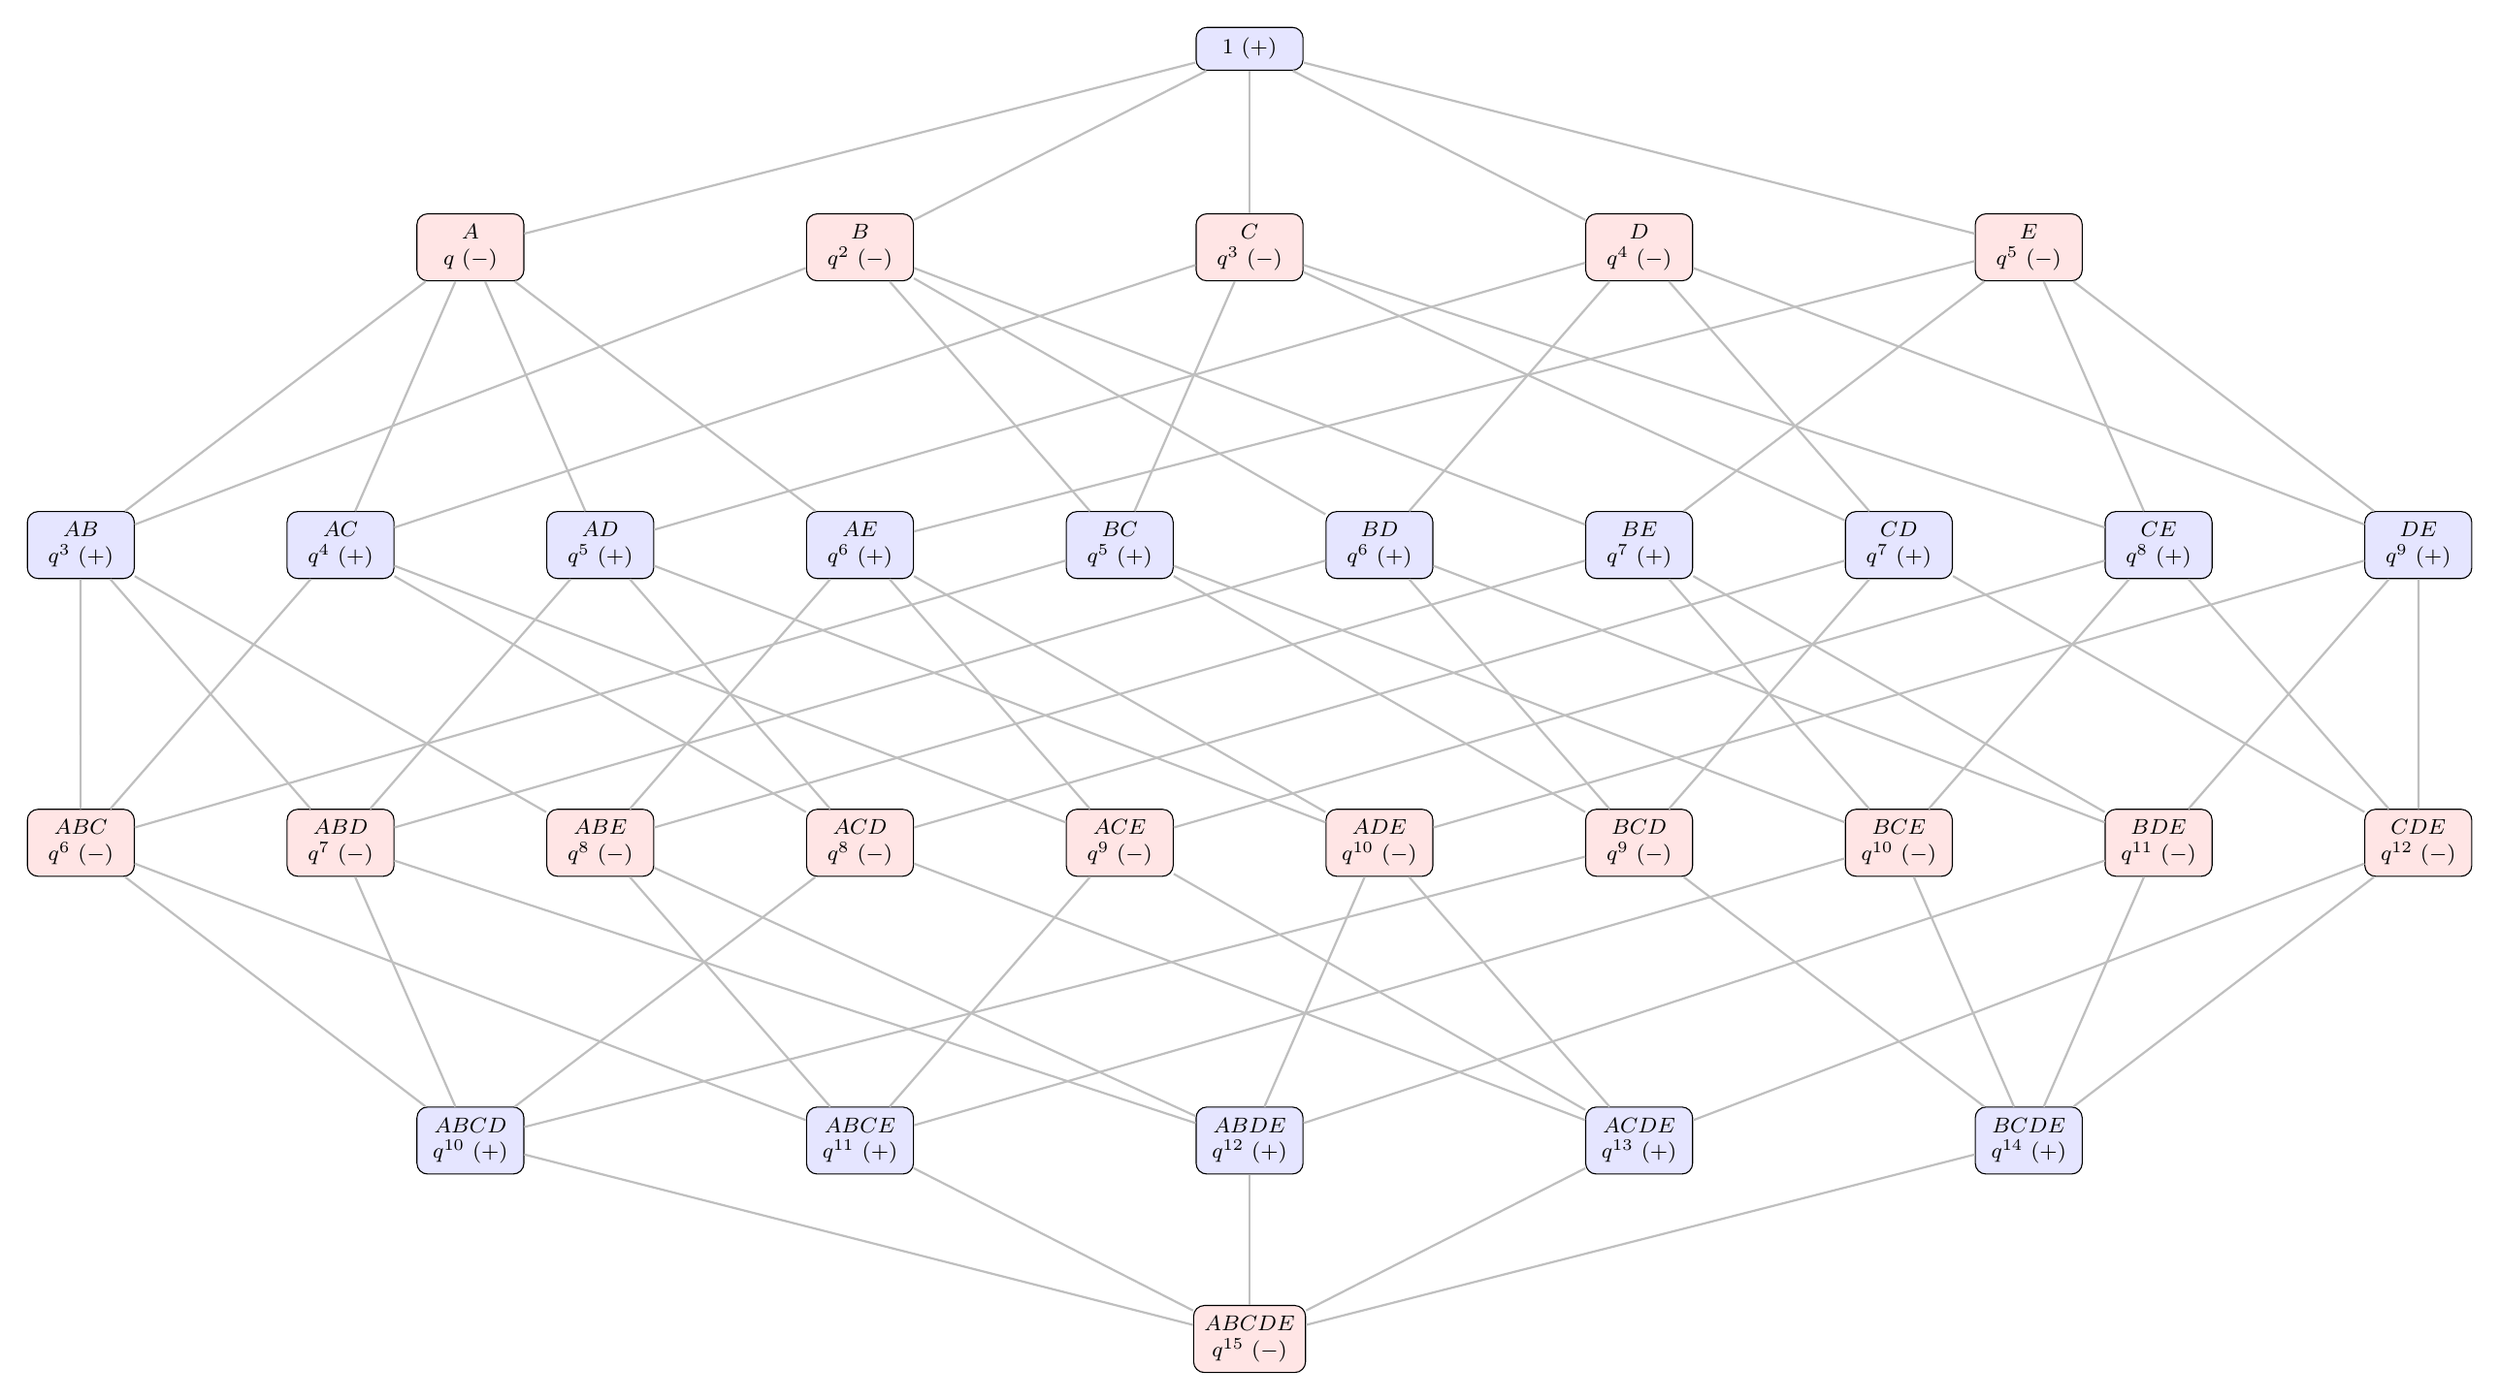
\begin{tikzpicture}[xscale=1.7, yscale=1.3]
				\node[pos node] (0) at (0, 0) {$1$ ($+$)};
				
				\node[neg node] (A) at (-6, -2) {$A$\\$q$ ($-$)\vphantom{$^2$}};
				\node[neg node] (B) at (-3, -2) {$B$\\$q^2$ ($-$)\vphantom{$^2$}};
				\node[neg node] (C) at (0, -2) {$C$\\$q^3$ ($-$)\vphantom{$^2$}};
				\node[neg node] (D) at (3, -2) {$D$\\$q^4$ ($-$)\vphantom{$^2$}};
				\node[neg node] (E) at (6, -2) {$E$\\$q^5$ ($-$)\vphantom{$^2$}};
				
				\node[pos node] (AB) at (-9, -5) {$AB$\\$q^3$ ($+$)};
				\node[pos node] (AC) at (-7, -5) {$AC$\\$q^4$ ($+$)};
				\node[pos node] (AD) at (-5, -5) {$AD$\\$q^5$ ($+$)};
				\node[pos node] (AE) at (-3, -5) {$AE$\\$q^6$ ($+$)};
				\node[pos node] (BC) at (-1, -5) {$BC$\\$q^5$ ($+$)};
				\node[pos node] (BD) at (1, -5) {$BD$\\$q^6$ ($+$)};
				\node[pos node] (BE) at (3, -5) {$BE$\\$q^7$ ($+$)};
				\node[pos node] (CD) at (5, -5) {$CD$\\$q^7$ ($+$)};
				\node[pos node] (CE) at (7, -5) {$CE$\\$q^8$ ($+$)};
				\node[pos node] (DE) at (9, -5) {$DE$\\$q^9$ ($+$)};
				
				\node[neg node] (ABC) at (-9, -8) {$ABC$\\$q^6$ ($-$)\vphantom{$^2$}};
				\node[neg node] (ABD) at (-7, -8) {$ABD$\\$q^7$ ($-$)\vphantom{$^2$}};
				\node[neg node] (ABE) at (-5, -8) {$ABE$\\$q^8$ ($-$)\vphantom{$^2$}};
				\node[neg node] (ACD) at (-3, -8) {$ACD$\\$q^8$ ($-$)\vphantom{$^2$}};
				\node[neg node] (ACE) at (-1, -8) {$ACE$\\$q^9$ ($-$)\vphantom{$^2$}};
				\node[neg node] (ADE) at (1, -8) {$ADE$\\$q^{10}$ ($-$)\vphantom{$^2$}};
				\node[neg node] (BCD) at (3, -8) {$BCD$\\$q^9$ ($-$)\vphantom{$^2$}};
				\node[neg node] (BCE) at (5, -8) {$BCE$\\$q^{10}$ ($-$)\vphantom{$^2$}};
				\node[neg node] (BDE) at (7, -8) {$BDE$\\$q^{11}$ ($-$)\vphantom{$^2$}};
				\node[neg node] (CDE) at (9, -8) {$CDE$\\$q^{12}$ ($-$)\vphantom{$^2$}};
				
				\node[pos node] (ABCD) at (-6, -11) {$ABCD$\\$q^{10}$ ($+$)};
				\node[pos node] (ABCE) at (-3, -11) {$ABCE$\\$q^{11}$ ($+$)};
				\node[pos node] (ABDE) at (0, -11) {$ABDE$\\$q^{12}$ ($+$)};
				\node[pos node] (ACDE) at (3, -11) {$ACDE$\\$q^{13}$ ($+$)};
				\node[pos node] (BCDE) at (6, -11) {$BCDE$\\$q^{14}$ ($+$)};
				
				\node[neg node] (ABCDE) at (0, -13) {$ABCDE$\\$q^{15}$ ($-$)\vphantom{$^2$}};
				
				\foreach \v in {A,B,C,D,E} \draw[edge style] (0) -- (\v);
				\foreach \u/\v in {A/AB,A/AC,A/AD,A/AE,B/AB,B/BC,B/BD,B/BE,C/AC,C/BC,C/CD,C/CE,D/AD,D/BD,D/CD,D/DE,E/AE,E/BE,E/CE,E/DE} \draw[edge style] (\u) -- (\v);
				\foreach \u/\v in {AB/ABC,AB/ABD,AB/ABE,AC/ABC,AC/ACD,AC/ACE,AD/ABD,AD/ACD,AD/ADE,AE/ABE,AE/ACE,AE/ADE,BC/ABC,BC/BCD,BC/BCE,BD/ABD,BD/BCD,BD/BDE,BE/ABE,BE/BCE,BE/BDE,CD/ACD,CD/BCD,CD/CDE,CE/ACE,CE/BCE,CE/CDE,DE/ADE,DE/BDE,DE/CDE} \draw[edge style] (\u) -- (\v);
				\foreach \u/\v in {ABC/ABCD,ABC/ABCE,ABD/ABCD,ABD/ABDE,ABE/ABCE,ABE/ABDE,ACD/ABCD,ACD/ACDE,ACE/ABCE,ACE/ACDE,ADE/ABDE,ADE/ACDE,BCD/ABCD,BCD/BCDE,BCE/ABCE,BCE/BCDE,BDE/ABDE,BDE/BCDE,CDE/ACDE,CDE/BCDE} \draw[edge style] (\u) -- (\v);
				\foreach \u in {ABCD,ABCE,ABDE,ACDE,BCDE} \draw[edge style] (\u) -- (ABCDE);
				
			\end{tikzpicture}
		}
	\end{center}
	
\end{document}